\subsection{Universal Gravitation}
The last section on mechanics will deal with gravity, starting with Newton's law of Universal Gravitation and looking at why this is consistent with Kepler's Laws of Planetary Motion.
\subsubsection{Newton's Law of Universal Gravitation}
From empirical observations, Newton posited the inverse-square law for gravity, where he claimed the force of gravity between two objects varied as the reciprocal of the square of the distance between the two.\\
\begin{center}
    \begin{asy}
        import geometry;
        size(8cm);
        
        draw(unitcircle);
        draw(shift(15, 0) * unitcircle);
        
        draw((0, -1.5)--(15, -1.5), linetype("8 8"), Arrows);
        draw((1,0)--(3,0), Arrow);
        draw((14,0)--(12,0), Arrow);
        
        label("$m_1$", (0, 1), N);
        label("$m_2$", (15, 1), N);
        label("$r_{12}$", (0, -1.5)--(15, -1.5), S);
        label("$\vec F_{12}$", (1,0)--(3,0), N);
        label("$\vec F_{21}$", (14,0)--(12,0), N);
    \end{asy}
\end{center}
Symbolically, if $m_1$ and $m_2$ are the masses of the two objects, $r_{12}$ is the distance between the two, and $\hat r_{12}$ is the unit vector in the direction from mass 1 to mass 2, then the gravitational force $\vec F_{21}$ on mass 2 due to mass 1 is:
\[
	\vec F = - \frac{Gm_1m_2}{r_{12}^2} \hat r_{12}
\]
The capital $G$ is not the acceleration due to gravity but is the universal gravitational constant that has the weird value of 6.674 $\cdot$ 10$^{-11}$ N$\cdot$m$^2$/kg$^2$. Notice that this formula also holds if you swap masses 1 and 2 - if we define $\hat r_{21}$ as the unit vector from mass 2 to mass 1 instead, so that $\hat r_{21} = - \hat r_{12}$, this still holds. As expected, the negative sign in front of the fraction is to ensure that this is an attractive force, since from real life we can clearly see that gravity pulls things together. 
\subsubsection{Gravitational Fields and Potential Energy}
Moving forward, we're going to work with different kinds of fields. Before moving on, I want to be clear as to what a field is - it's the assignment of some value to every point in space. Mostly, we're going to look at vector fields and scalar fields - fields where a vector/scalar are assigned to every point. The first ones we'll encounter in physics are the gravitational field and the gravitational potential. \\
Consider placing a very small test point particle $m_0$ amongst a collection of masses. These masses exert a gravitational force $\vec F_{net}$ on the particle:
\[
	\vec F_{net} = \sum_i \vec F_i = \sum_i -\frac{Gm_0m_i}{r_i^2}\hat r_i
\]
(For clarity - I'm using $m_i$ as the mass of the $i$th particle, $r_i$ for the distance between $m_0$ and $m_i$, and $\hat r_i$ as the unit vector in the direction from $m_0$ to $m_i$.)\\
Now, define the gravitational field at the position of the test mass $m_0$ as the net gravitational force divided by the mass of the small test particle:
\[
	\vec g = \frac{\vec F_{net}}{m_0} = \sum_i -\frac{Gm_i}{r_i^2}\hat r_i
\]
Notice for a single point mass, then, we have the gravitational field $\vec g = -\frac{Gm_i}{r^2}\hat r$ where $r$ is the distance from the point mass and $\hat r$ is just radially outward from the mass. However, more likely than not we are going to encounter continuous distributions of mass, which will require integration and superposing infinitely many small gravitational fields to create the total field. Here, we're going to derive the gravitational field due to a thin ring of mass and for a spherical shell. \\
\begin{center}
    \begin{asy}
        import three;
        size(6cm);
        triple eye = (7, 8, 5);
        currentprojection = perspective(eye);
        triple center = (0, 0, 0);
        real R = 1, y = 2;
        draw(circle(center, R, Z));
        dot((0, 0, y));
        real dqAngle = -20, dqDelta = 6;
        draw(arc(center, R,
                90, dqAngle - dqDelta,
                90, dqAngle + dqDelta), linewidth(2));
        draw(dir(90, dqAngle) -- (0, 0, y), linetype("6 6"));
        triple radiusPt = R * dir(90, 170);
        draw((0, 0, 0)--radiusPt, gray(0.2));
        draw((0, 0, 0)--(0, 0, y), gray(0.2));
        
        label("$M$", (0, R, 0), dir(-90));
        label("$m_0$", (0, 0, y), dir(130));
        label("$dM$", dir(90, dqAngle), dir(200));
        label("$R$", radiusPt/2, dir(-40));
        label("$y$", (0, 0, y/2), dir(0));
    \end{asy}
\end{center}
First, let's consider a uniform ring of mass $M$ and radius $R$, and for simplicity let's use a test mass $m_0$ on the axis of symmetry of the ring, at a distance of $y$ above the center. This ring has a linear mass density $\lambda = \frac{M}{2\pi R}$. We can consider dividing the ring into infinitely many tiny arcs, with length $ds = R \, d\theta$. The mass of this piece can then be shown to be $dm = \lambda R \, d\theta$. \\
From this, we conclude the magnitude of the force on the test mass from this small arc, $dF$, is
\[
    dF = \frac{Gm_0 \,dm}{R^2 + y^2}
\]
Note that the radial components of the force will cancel each other out by symmetry, so it suffices to consider the components of the force in the $y$-direction, $dF_y$:
\[
    dF_y = -\frac{Gm_0 \, dm}{R^2 + y^2} \cdot \frac{y}{\sqrt{R^2+y^2}} = \frac{Gm_0 \, dm \, y}{(R^2 + y^2)^{3/2}}.
\]
The negative sign is present since gravity is an attractive force. We can now integrate over all the small bits of mass: 
\begin{align*}
    F &= \int_0^{2\pi} dF_y \\
    &= \int_0^{2\pi} -\frac{Gm_0 \, dm \, y}{(R^2 + y^2)^{3/2}} \\
    &= \int_0^{2\pi} -\frac{Gm_0y \lambda R \, d \theta}{(R^2 + y^2)^{3/2}}\\
    &= -\frac{Gm_0My}{(R^2 + y^2)^{3/2}}.
\end{align*}
The force is directed in the negative $y$-direction, and thus the force is
\[
    \vec F = -\frac{Gm_0My}{(R^2 + y^2)^{3/2}}\hat y
\]
To find the gravitational field along the axis at any distance from the center $y$, we simply use our definition to find:
\[
    \vec g = \frac{GMy}{(R^2 + y^2)^{3/2}}\hat y.
\]
\begin{center}
    \begin{asy}
        import solids;
        import three;
        size(8cm);
        
        currentprojection=orthographic(0.7, -4, 1);
        currentlight=nolight;
        triple center = (0,0,0);
        triple ringctr = (0.5, 0, 0);
        real R=1, RS=0.7, inc=100, lat=45, lon=45, tlat=50, tlon=100;
        dot(center);
        real r = 2;
        dot(ringctr);
        revolution Earth=sphere(center, R);  
        
        draw(surface(Earth), surfacepen=white+opacity(.1), meshpen=0.7*black);
        draw(arc(ringctr, sqrt(3)/2, 0, 90, 180, 270), linewidth(2));
        draw(arc(ringctr, sqrt(3)/2, 180, 270, 0, 90), linewidth(2)+linetype("4 4"));
        dot((r, 0, 0));

        draw((0,0,0)--(r, 0, 0));
        draw(center--(0.5, 0, sqrt(3)/2));
        label("$R$", (0.25, 0, sqrt(3)/4), dir(120));
        label("$dM$", (0.5, 0, sqrt(3)/2), dir(40)*1.5);
        label("$\theta$", center, dir(30)*2);
        label("$r$", (r*0.75, 0, 0), dir(90));
        label("$m_0$", (r, 0, 0), dir(50));
    \end{asy}
\end{center}
From here, we can proceed to find the gravitational field of a uniform thin spherical shell of mass $M$ and radius $R$, making the surface density $\sigma = \frac{M}{4\pi R^2}$. Consider a test mass $m_0$, a distance $r$ away from the center of the sphere. We can split the sphere into many rings and use a scanning variable $\theta$ that represents the angle between the line joining the center to the edge of the ring and the horizontal. The surface area of each ring $dA = 2\pi R^2 \sin \theta \, d\theta$ (as seen before in the moment of inertia calculation), so then mass of each ring, $dm$, can be seen to be $dm = 2\pi \sigma R^2 \sin \theta \, d\theta$. We can then plug straight back into the formula for a ring to get: 
\[
    dF = \frac{Gm_0(r-R\cos \theta)\, dm}{((R\sin \theta)^2 + (r-R\cos \theta)^2)^{3/2}} = \frac{2Gm_0R^2 \pi \sigma (r-R\cos \theta) \sin \theta \, d\theta}{((R\sin \theta)^2 + (r-R\cos \theta)^2)^{3/2}}
\]
We integrate with respect to $\theta$ from $0$ to $\pi$, and simplify as much as possible: 
\begin{align*}
    F &= \int_0^\pi \frac{2Gm_0R^2 \pi \sigma (r-R\cos \theta) \sin \theta \, d\theta}{((R\sin \theta)^2 + (r-R\cos \theta)^2)^{3/2}}\\
    &= Gm_0\pi\sigma \int_0^\pi \frac{2R^2 (r-R\cos \theta) \sin \theta \, d\theta}{(R^2 + r^2 - 2rR\cos \theta)^{3/2}}
\end{align*}
Let $u = R^2 + r^2 - 2rR\cos \theta$, and $du = 2rR \sin \theta \, d\theta$, which changes the bounds to $(r-R)^2$ to $(r+R)^2$. From this, we also get that $\cos \theta = \frac{R^2+r^2-u}{2Rr}$ and gives
\begin{align*}
    F &= Gm_0\pi\sigma \int_{(r-R)^2}^{(r+R)^2} \frac{R}{r} \left(r-\frac{R^2+r^2-u}{2r}\right) u^{-\frac{3}{2}}\, du \\
    &= \frac{Gm_0\pi\sigma R}{2r^2} \int_{(r-R)^2}^{(r+R)^2} (r^2-R^2+u) u^{-\frac{3}{2}}\, du \\
    &= \frac{Gm_0\pi\sigma R}{2r^2} \int_{(r-R)^2}^{(r+R)^2} (r^2-R^2)u^{-\frac{3}{2}} + u^{-\frac{1}{2}}\, du \\
    &= \frac{Gm_0\pi\sigma R}{2r^2} (-2(r^2-R^2)u^{-\frac{1}{2}} + 2u^{\frac{1}{2}}) \Big|_{(r-R)^2}^{(r+R)^2} \\
    &= \frac{Gm_0\pi\sigma R}{r^2} ((R^2-r^2)u^{-\frac{1}{2}} + u^{\frac{1}{2}}) \Big|_{(r-R)^2}^{(r+R)^2}\\
\end{align*}
\textbf{Case 1: Outside the Shell} \newline
Assume now that $r > R$, so $r - R> 0$. Evaluating, we have
\begin{align*}
    F &= \frac{Gm_0\pi\sigma R}{r^2} \left(\frac{R^2-r^2}{r+R} + R+r - \frac{R^2-r^2}{r-R} - (r - R)\right) \\
    &= \frac{Gm_0\pi\sigma R}{r^2} (R-r + R+r + R+ r + R -r)\\
    &= \frac{Gm_0\pi\sigma 4R^2}{r^2} \\
    &= \frac{Gm_0Q}{r^2} 
\end{align*}
From this, we see that 
\[
    \vec g = \frac{GM}{r^2}\hat r
\]
where $\hat r$ is the unit vector radially outward from the center of the sphere to the point charge. \\ 
\textbf{Case 2: Inside the Shell} \\
Assume now that $r < R$, so $R - r> 0$. Evaluating, we have
\begin{align*}
    F &= \frac{Gm_0\pi\sigma R}{r^2} \left(\frac{R^2-r^2}{r+R} + R+r - \frac{R^2-r^2}{R-r} - (R-r)\right) \\
    &= \frac{Gm_0\pi\sigma R}{r^2} (R-r + R+r - R - r -R + r)\\
    &= 0
\end{align*}
and clearly $\vec g = 0$. Notice that outside the shell, the field is exactly the same as if the shell was essentially a point mass, and on the inside, it's zero. This is a result known as the Shell Theorem. \\
Another field that we will investigate is a scalar field, the potential energy field. First, let's look at the gravitational potential energy of a mass $m_0$ brought from arbitrarily far away (so, basically infinity) to a distance $r$ away from a mass $M$. Assuming the potential energy at infinity is zero, the potential energy function $U(r)$ is then:
\[
	U = - \int_r^{\infty} F \, dr = - \int_r^{\infty} -\frac{Gm_0M}{r^2} \, dr = -\frac{Gm_0M}{r}
\]
This also follows the principles of superposition that is true for gravitational fields, but direction need not be taken into account because energy is a scalar. For reference, here are the potential energies of a test particle $m_0$ near the ring and shell:
\[
	U = -\frac{GMm_0}{\sqrt{R^2 + y^2}} \quad U = -\frac{Gm_0M}{r}
\]
\subsubsection{Kepler's Laws of Planetary Motion}
Before Newton, Kepler proposed three laws of planetary motion from empirical data of the positions of astronomical bodies as they orbited the sun. These are the laws Kepler proposed: \\
1. All planets orbit around a sun in elliptical orbits with the sun at one focus of the ellipse.\\
2. Planets sweep out equal-sized areas in equal time intervals. \\
3. The square of the period of a planet's orbit is proportional to the cube of the semi-major axis of the planet's orbit: more specifically, 
\[
	T^2 = \frac{4\pi^2}{GM} a^3
\]
where $M$ is the mass of the sun. \\
% \section*{Appendix A: Proof of Kepler's Laws}
% \addcontentsline{toc}{section}{Appendix A: Proof of Kepler's Laws}
% As a reminder, here is a restatement of Kepler's Laws:\\
% 1. All planets orbit around a sun in elliptical orbits with the sun at one focus of the ellipse.\\
% 2. Planets sweep out equal-sized areas in equal time intervals. \\
% 3. The square of the period of a planet's orbit around a mass $M$ is proportional to the cube of the semi-major axis of the planet's orbit: more specifically, 
% \[
% 	T^2 = \frac{4\pi^2}{GM} a^3
% \]
The first and third statements follow from Newton's Law of Universal Gravitation, but the second is essentially a disguised conservation of angular momentum (see the problems from Rotation!). We're going to prove these two using Newton's Law of Universal Gravitation and Newton's Second Law of Motion. \\
\begin{center}
	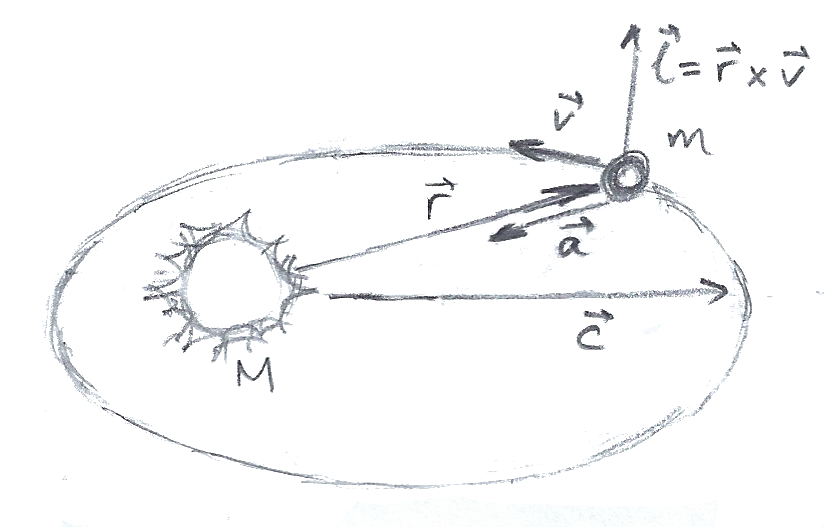
\includegraphics[width=0.5\textwidth]{images/mechintro/kepler-1.png}\\
\end{center}
If a satellite of mass $m$ is orbiting around a mass $M$, the force $\vec F = - \frac{GmM}{r^2} \hat r$ where $\hat r$ and $r$ are varying with time. Because of this, notice that $\vec a =  - \frac{GM}{r^2} \hat r$ from Newton's Second Law. The position $\vec r$ and $\vec a$ are then always in the same direction. \\
Assuming no other forces act on the system, the orbital angular momentum $\vec L = \vec r \times m \vec v$ is constant. We're more interested in the fact that the cross product $\vec r \times \vec v$ is also a constant, so we're going to denote this by $\vec l$. But what exactly is $\vec l$? We can do this explicitly:
\begin{align*}
	\vec l &= \vec r \times \vec v \\
	&= \vec r \times \dv{\vec r}{t}\\
	&= r \hat r \times \dv{}{t}(r \hat r)\\
	&= r \hat r \times (r' \hat r + r \hat r')\\
	&= r^2(\hat r \times \hat r')\\
\end{align*}
We're going to do something a little contrived: what happens when we take $\vec a \times \vec l$? We can use the triple vector product identity to help us out, and the fact that we've decomposed everything into unit vectors with magnitude 1:
\begin{align*}
	\vec a \times \vec l &=  - \frac{GM}{r^2} \hat r \times r^2 (\hat r \times \hat r')\\
	&= -GM [ \hat r (\hat r \cdot \hat r') - \hat r' (\hat r \cdot \hat r) ]\\
	&= GM \hat r'
\end{align*}
The first dot product in parentheses is zero - the derivative of a unit vector is always perpendicular to the original. If you're not convinced, look at $\hat r$ and $\hat \theta$ when we derived circular motion - $\hat \theta$ is proportional to the derivative of $\hat r$, and $\hat \theta \cdot \hat r = 0$. \\
Since we know how $\vec a \times \vec l$, we can find $\vec v \times \vec l$. Considering that 
\[
	\dv{}{t} (\vec v \times \vec l) = \dv {\vec v}{t} \times l + \vec v \times \dv{\vec l}{t} = \vec a \times \vec l + \vec v \times \vec 0 = \vec a \times \vec l
\]
we can integrate to find $\vec v \times \vec l = GM \hat r + \vec c$ for some constant vector $\vec c$. \\
We have one more contrived step to take: consider $\vec r \cdot (\vec v \times \vec l)$. We can expand it as follows:
\begin{align*}
	\vec r \cdot (\vec v \times \vec l) &= \vec r \cdot (GM \hat r + \vec c) \\
	&= GM (\vec r \cdot \hat r) + \vec r \cdot \hat c\\
	&= GMr + rc \cos \theta
\end{align*}
where $\theta$ is the angle between $\vec r$ and $\vec c$. On the other hand, since this is a scalar triple product, $\vec r \cdot (\vec v \times \vec l) = \vec l \cdot (\vec r \times \vec v) = \vec l \cdot \vec l = l^2$. Therefore, 
\[
	l^2 = GMr + rc \cos \theta
\]
\[
	r = \frac{l^2}{GM + c \cos \theta} = \frac{\frac{l^2}{GM}}{1 + \frac{c}{GM} \cos \theta}
\]
That is the polar equation for an ellipse, centered at one of its foci (if you might recall from the conics unit), and this gives Kepler's First Law.\\
\begin{center}
	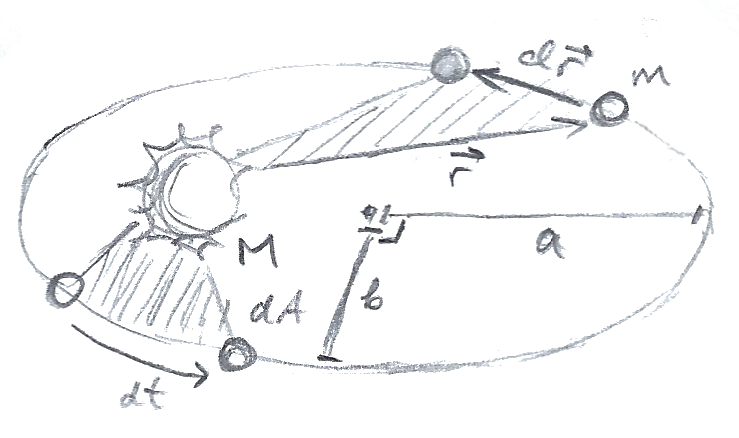
\includegraphics[width=0.5\textwidth]{images/mechintro/kepler-2.png}\\
\end{center}
For Kepler's Second Law, we reuse the fact that $\vec l = \vec r \times \vec v$ is a constant. Consider a small triangular area $dA$ swept out in a time $dt$ by a satellite. This area $dA = \frac{1}{2}| \vec r \times d\vec r |$, where $d\vec r$ is the displacement of the satellite. Dividing by $dt$ gives $\dv{A}{t} = \frac{1}{2} \left| \vec r \times \dv{\vec r}{t} \right| = \frac{1}{2} \left| \vec r \times \vec v \right| = \frac{1}{2} l$. Since $\vec l$ is constant, we have that the area swept out per unit time is constant, so the area swept out by a satellite in a given time interval is also a constant. \\
Using this, we can prove Kepler's Third Law. The rate at which area is swept out is $\dv{A}{t} = \frac{1}{2} l$ by Kepler's Second Law, but since this is constant it's also equal to the total area of the elliptical orbit over the period of the motion. Letting $a$ and $b$ be the lengths of the semi-major and semi-minor axes, we have 
\[
	\dv{A}{t} = \frac{\pi a b}{T} = \frac{1}{2}l
\]
From this, we see that 
\[
	T = \frac{2\pi a b}{l} \rightarrow T^2 = \frac{4\pi^2 a^2 b^2}{l^2}
\]
I'm going to gloss over this part a little bit - but recall that an ellipse in polar coordinates is defined by its eccentricity $e$ and the distance from the focus to the directrix $d$. The computation is extremely messy, but it can be shown (with great effort) that the numerator of the polar equation $ed = \frac{b^2}{a}$. In this case, then, $\frac{l^2}{GM} = \frac{b^2}{a}$, which is equivalent to $\frac{b^2}{l^2} = \frac{a}{GM}$. We can plug this back in to get
\[
	T^2 = \frac{4\pi^2}{GM}a^3
\]
This shows Kepler's Third Law. Usually, however, we won't work with actual elliptical orbits - most of the time we will just deal with simplified circular orbits, where the semi-major axis is just the radius of the circle. 
These equations hold true in general for satellites orbiting around large masses, if the satellite's mass is negligible - otherwise, one must consider orbit around the center of mass and use the total mass for Kepler's Third Law. We will see why this is as a problem at the end of the chapter.
\subsubsection{Summary and Problems} 
Using Newton's Law of Gravitation and our knowledge of mechanics up to this point, we derived Kepler's Laws and we can now apply them in these problems. As a result of Newton's Law of Gravitation, we were also able to derive a gravitational field which we will calculate for a few setups. We can also look at the potential energy of gravitational fields, which we will also explore a little. \\

\noindent\textbf{Problems:}\\
1. (1 $\bigstar$) Given that the mean period of the Moon's orbit is 27.3 days, the mean orbital radius of the Moon around the Earth is 385,000 km, and the value of $G$, approximate the mass of the Earth to be about 6.07$\cdot$10$^{24}$ kg. \\
2. (2 $\bigstar$, $\spadesuit$) Two particles, each of mass $M$, are fixed in position on the $y$-axis at $y = +a$ and $y = -a$. Show that on the $x-$axis, the maximum value of $g$ for the gravitational field occurs at points $x = \pm a/\sqrt{2}$. \\
3. (3 $\bigstar$) An object is projected vertically from the surface of Earth at less than the escape speed. Show that the maximum height $H$ reached by the object is $H = \frac{R_EH'}{R_E - H'}$, where $H'$ is the height that it would reach if the gravitational field were constant, and $R_E$ is the radius of the Earth. Notice that for large values of the launch velocity for a projectile, this model is more precise if significant fluctuations in the gravitational field are observed over the course of the object's flight.\\
4. (4 $\bigstar$, $\spadesuit$) A uniform thin rod of mass $M$ and length $L$ lies on the $+x$-axis with one end at the origin. Consider an element of the rod of length $dx$, and mass $dm$, at point $x$, where $0<x<L$. a) Show that this element produces a gravitational field $dg_{x}$ at a point $x_0$ on the $x-$axis in the region $x_0 > L$ is given by $dg_{x} = -\frac{GM}{L(x_0-x)^2}$. b) Show that the total gravitational field at the point $x_0$ due to the rod is $g = \frac{GM}{x_0(x_0-L)}$. c) Show that for $x_0 >> L$, the field of the rod approximates the field of a point particle of mass $M$ at $x = 0$. d) Using a similar method, compute the gravitational potential energy of a mass $m_0$ at a position $x_0$ to be $U = -\frac{GMm_0}{L} \ln\left(\frac{x_0+L/2}{x_0-L/2}\right)$.\\
5. (3 $\bigstar$) In a binary star system, two stars follow circular orbits about their common center of mass. If the stars have masses $m_1$ and $m_2$ and are separated by a distance $r$, show that the period of rotation is related to $r$ by $T^2 = \frac{4\pi^2}{G(m_1+m_2)}r^3$. \\
6. (2 $\bigstar$) Four identical planets are arranged in a square of side length $a$. If the mass of each planet is $M$, show that the speed of each planet is $v = \sqrt{\frac{GM}{a}\left(\frac{\sqrt{2}}{4} + 1 \right)}$ if they are to orbit their common center under the influence of their mutual attraction.\\
7. (3 $\bigstar$) Two particles of masses $m_1$ and $m_2$ are released from rest at a large separation distance. Show that their speeds $v_1$ and $v_2$ when their separation distance is $r$ are $v_1 = \sqrt{\frac{2Gm_2^2}{r(m_1+m_2)}}$ and $v_2 = \sqrt{\frac{2Gm_1^2}{r(m_1+m_2)}}$.
\pagebreak